\documentclass[,a4paper]{article}
\usepackage{geometry}
\geometry{a4paper,left=35mm,right=35mm, top=25mm, bottom=25mm}
\usepackage[T1]{fontenc}
\usepackage{lmodern}
\usepackage{amssymb,amsmath}
\usepackage{ifxetex,ifluatex}
\usepackage{fixltx2e} % provides \textsubscript
% use microtype if available
\IfFileExists{microtype.sty}{\usepackage{microtype}}{}
\ifnum 0\ifxetex 1\fi\ifluatex 1\fi=0 % if pdftex
  \usepackage[utf8]{inputenc}
\else % if luatex or xelatex
  \usepackage{fontspec}
  \ifxetex
    \usepackage{xltxtra,xunicode}
  \fi
  \defaultfontfeatures{Mapping=tex-text,Scale=MatchLowercase}
  \newcommand{\euro}{€}
\fi
\usepackage{color}
\usepackage{fancyvrb}
\DefineShortVerb[commandchars=\\\{\}]{\|}
\DefineVerbatimEnvironment{Highlighting}{Verbatim}{commandchars=\\\{\}}
% Add ',fontsize=\small' for more characters per line
\newenvironment{Shaded}{}{}
\newcommand{\KeywordTok}[1]{\textcolor[rgb]{0.00,0.44,0.13}{\textbf{{#1}}}}
\newcommand{\DataTypeTok}[1]{\textcolor[rgb]{0.56,0.13,0.00}{{#1}}}
\newcommand{\DecValTok}[1]{\textcolor[rgb]{0.25,0.63,0.44}{{#1}}}
\newcommand{\BaseNTok}[1]{\textcolor[rgb]{0.25,0.63,0.44}{{#1}}}
\newcommand{\FloatTok}[1]{\textcolor[rgb]{0.25,0.63,0.44}{{#1}}}
\newcommand{\CharTok}[1]{\textcolor[rgb]{0.25,0.44,0.63}{{#1}}}
\newcommand{\StringTok}[1]{\textcolor[rgb]{0.25,0.44,0.63}{{#1}}}
\newcommand{\CommentTok}[1]{\textcolor[rgb]{0.38,0.63,0.69}{\textit{{#1}}}}
\newcommand{\OtherTok}[1]{\textcolor[rgb]{0.00,0.44,0.13}{{#1}}}
\newcommand{\AlertTok}[1]{\textcolor[rgb]{1.00,0.00,0.00}{\textbf{{#1}}}}
\newcommand{\FunctionTok}[1]{\textcolor[rgb]{0.02,0.16,0.49}{{#1}}}
\newcommand{\RegionMarkerTok}[1]{{#1}}
\newcommand{\ErrorTok}[1]{\textcolor[rgb]{1.00,0.00,0.00}{\textbf{{#1}}}}
\newcommand{\NormalTok}[1]{{#1}}
% Redefine labelwidth for lists; otherwise, the enumerate package will cause
% markers to extend beyond the left margin.
\makeatletter\AtBeginDocument{%
  \renewcommand{\@listi}
    {\setlength{\labelwidth}{4em}}
}\makeatother
\usepackage{enumerate}
\usepackage{graphicx}
% We will generate all images so they have a width \maxwidth. This means
% that they will get their normal width if they fit onto the page, but
% are scaled down if they would overflow the margins.
\makeatletter
\def\maxwidth{\ifdim\Gin@nat@width>\linewidth\linewidth
\else\Gin@nat@width\fi}
\makeatother
\let\Oldincludegraphics\includegraphics
\renewcommand{\includegraphics}[1]{\Oldincludegraphics[width=\maxwidth]{#1}}
\ifxetex
  \usepackage[setpagesize=false, % page size defined by xetex
              unicode=false, % unicode breaks when used with xetex
              xetex]{hyperref}
\else
  \usepackage[unicode=true]{hyperref}
\fi
\hypersetup{breaklinks=true,
            bookmarks=true,
            pdfauthor={OParl Team - http://oparl.de/},
            pdftitle={OParl Schnittstellen-Spezifikation (Entwurf)},
            colorlinks=true,
            urlcolor=blue,
            linkcolor=magenta,
            pdfborder={0 0 0}}
\setlength{\parindent}{0pt}
\setlength{\parskip}{6pt plus 2pt minus 1pt}
\setlength{\emergencystretch}{3em}  % prevent overfull lines
\setcounter{secnumdepth}{0}

\title{OParl Schnittstellen-Spezifikation (Entwurf)}
\author{OParl Team - http://oparl.de/}
\date{}

\begin{document}
\maketitle

Lizenz: Creative Commons CC-BY-SA

\section{Einleitung}

Dieses Dokument wird bei seiner Fertigstellung die Spezifikation des
OParl Schnittstellen-Standards für parlamentarische Informationssysteme
(Ratsinformationssysteme, RIS) darstellen. Es dient damit als Grundlage
für die Implementierung von OParl-konformen Server- und
Clientanwendungen.

\subsection{Motivationen für den standardisierten Datenzugriff}

Die Gründe, warum Betreiber von parlamentarischen Informationssystemen
den Zugriff darauf über eine standardisierte Schnittstelle ermöglichen
sollten, können vielfältig sein.

Ein zentrales Argument ist die Verpflichtung der Parlamente gegenüber
der Bevölkerung, diese über die Fortschritte der parlamentarischen
Arbeit zu informieren und auf dem Laufenden zu halten. Ein erster
Schritt, der Bevölkerung Einblicke in die Arbeit und Zugriff auf
Dokumente zu gewähren, ist vielerorts in den letzten Jahren durch
Einführung von Ratsinformationssystemen mit anonymem, lesenden Zugriff
über das World Wide Web gemacht worden.

Die damit eingeschlagene Richtung konsequent weiter zu gehen, bedeutet,
die Daten der parlamentarischen Informationssystemen gänzlich offen zu
legen, sofern die Inhalte es erlauben. Es bedeutet, die Daten und
Inhalte so universell weiterverwendbar und so barrierearm wie möglich
anzubieten, dass jegliche weitere Verwendung durch Dritte technisch
möglich ist. Der seit einiger Zeit etablierte Begriff für dieses Prinzip
heißt ``Open Data''.

Das Interesse an parlamentarischen Informationen und an Anwendungen, die
diese nutzbar und auswertbar machen, ist offensichtlich vorhanden. Die
Entwickler der alternativen Ratsinformationssysteme wie Frankfurt
Gestalten{[}14{]}, Offenes Köln{[}15{]} oder der
OpenRuhr:RIS-Instanzen{[}16{]} wissen zu berichten, wie viel Interesse
den Projekten gerade aus Orten entgegen gebracht wird, in denen
derartige Systeme noch nicht verfügbar sind.

Die Anwendungsmöglichkeiten für parlamentarische Informationen, wenn sie
über eine Schnittstelle schnell und einfach abgerufen werden können,
sind vielfältig. Beispiele könnten sein:

\begin{itemize}
\item
  Apps für den Abruf auf mobilen Endgeräten
\item
  Möglichkeiten zur Wiedergabe für Nutzerinnen und Nutzer mit
  Beeinträchtigung des Sehvermögens
\item
  Alternative und erweiterte Suchmöglichkeiten in Inhalten
\item
  Auswertung und Analyse von Themen, Inhalten, Sprache etc.
\item
  Benachrichtigungsfunktionen beim Erscheinen bestimmte Inhalte
\end{itemize}

Die Standardisierung dieses Zugriffs über die Grenzen einzelner Systeme
hinweg erlaubt zudem, diese Entwicklungen grenzüberschreitend zu denken.
Damit steigt nicht nur die potenzielle Nutzerschaft einzelner
Entwicklungen. Auch das Potenzial für Kooperationen zwischen
Anwendungsentwicklern wächst.

Darüber hinaus sind auch Motivationen innerhalb von Organisationen und
Körperschaften erkennbar. So sollen parlamentarische Informationssysteme
vielerorts in verschiedenste Prozesse und heterogene Systemlandschaften
integriert werden. Durch eine einheitliche Schnittstelle bieten sich
effiziente Möglichkeiten zur Integration der Daten in anderen Systeme,
wie beispielsweise Web-Portale.

\subsection{Funktionsumfang der OParl-Schnittstelle}

Die vorliegende Spezifikation soll eine Webservice-Schnittstelle
definieren, die den anonymen und lesenden Zugriff auf öffentliche
Inhalte aus Parlamentarischen Informationssystemen ermöglicht. Die
Zugriffe erfolgen über das Hypertext Transfer Protocol (HTTP). Daten
werden als JSON oder als JSONP ausgeliefert.

Die Spezifikation wird obligatorische Bestandteile (MUSS) und optionale
Bestandteile (KANN) haben. Der tatsächliche Funktionsumfang kann daher
zwischen den Implementierungen variieren.

\subsection{Status}

Die Spezifikation befindet sich in Arbeit. Das Dokument enthält
entsprechend viele Ungenauigkeiten und Hinweise auf offene
Fragestellungen.

\subsection{Was ist OParl?}

\subsection{Zielsetzung von OParl}

\begin{itemize}
\item
  Nutzen für Kommunen, Bürger, politische Parteien
\item
  Nutzen für Anbieter von RIS-Pflegesoftware
\item
  Nutzen für Anbieter von RIS-Darstellungssoftware
\item
  Nutzen für Open Data Initiativen
\item
  Nutzen für die Wissenschaft
\item
  Linked Data erwähnen
\end{itemize}

\subsection{Werdegang von OParl 1.0}

Stichpunkte:

\begin{itemize}
\item
  \begin{enumerate}[1.]
  \setcounter{enumi}{16}
  \item
    und 18. November 2012: Die Open Knowledge Foundation Deutschland
    veranstaltet in den Räumen der Heinrich-Böll-Stiftung in Berlin
    einen Workshop für Entwickler von Anwendungen, die einen
    gesellschaftlichen Nutzen bringen sollen. Hier ist VITAKO, die
    Bundes-Arbeitsgemeinschaft der Kommunalen IT-Dienstleister, als
    Sponsor engagiert. Die Geschäftsführerin, Dr.~Marianne Wulff, ist
    persönlich vor Ort. Auch das Projekt Offenes Köln wird in einem
    Vortrag von Marian Steinbach präsentiert. Es kommt zum Austausch
    über die Frage, wie das Prinzip der offenen Ratsinformationen
    effektiv auf weitere Kommunen ausgeweitet werden könnte.
  \end{enumerate}
\item
  \begin{enumerate}[1.]
  \setcounter{enumi}{5}
  \item
    Dezember 2012: Anhörung im Landtag NRW in Düsseldorf zu einer
    Open-Data-Strategie der Landesregierung, wo Jens Klessmann und
    Marian Steinbach als Sachverständige gehört werden. Danach Gespräch
    über Möglichkeiten der Standardisierung offener
    Ratsinformationssysteme.
  \end{enumerate}
\item
  Dezember 2012: Dr.~Marianne Wulff, Jens Klessmann und Marian Steinbach
  beginnen mit der Abstimmung über einen Workshop mit Vertreterinnen und
  Vertretern von Kommunen, kommunalen IT-Dienstleistern, RIS-Anbietern
  und Zivilgesellschaft. Ziel: Die Bereitschaft zur Zusammenarbeit an
  einem gemeinsamen Standard ermitteln. Unterdessen beginnt Marian
  Steinbach mit der Formulierung eines Standard-Entwurfs als
  Diskussionsgrundlage. Der Entwurf wird von Beginn an öffentlich auf
  GitHub.com bereit gestellt.
\item
  \begin{enumerate}[1.]
  \setcounter{enumi}{16}
  \item
    April 2013: Insgesamt 30 Teilnehmer versammeln sich in Köln, um sich
    in einem ersten Treffen über Ziele und Chancen einer
    Standardisierung für offene Ratsinformationen auszutauschen. Als
    Ergebnis wird ein großes Interesse an der weiteren Zusammenarbeit
    auf Basis des vorliegenden Standardentwurfs festgestellt. Als Termin
    für die Fertigstellung der ersten Version der Spezifikation wird der
    30. Juni 2013 festgelegt. Die Initiatoren präsentieren den
    Anwesenden hier erstmals den Namen ``OParl'', der künftig als Marke
    für die Bemühungen der Gruppe stehen soll.
  \end{enumerate}
\item
  \begin{enumerate}[1.]
  \setcounter{enumi}{21}
  \item
    Januar 2014: Nachdem sich die verteilte Zusammenarbeit am
    Standard-Entwurf seit April 2013 als nicht zielführend erwiesen hat,
    laden Jens Klessmann und Marian Steinbach und VITAKO zu einem
    eintägigen OParl-Workshop in Bielefeld ein. Das Ziel ist, die
    Spezifikation so weit wie möglich voran zu treiben und eine gute
    Basis für die baldige Fertigstellung zu legen.
  \end{enumerate}
\end{itemize}

\subsection{Zukunft von OParl}

\begin{itemize}
\item
  Verfeinerung, Lücken schliessen
\item
  Globalisierung
\item
  Erweiterung über die kommunale Ebene hinaus (Land, Bund)
\item
  Vereinheitlichung von Kategorien (Drucksachentypen, Arten von Gremien)
\item
  Erweiterung von Personendaten, z.B. mit Social Media URLs
\item
  Mehr Abfragekriterien
\item
  Suchfunktionen (Volltextsuche)
\item
  Abstimmungsverhalten und maschinenlesbare Protokolle
\end{itemize}

\subsection{Nomenklatur der Spezifikation und Satzkonventionen}

\subsubsection{MÜSSEN, SOLLEN und KÖNNEN bzw. ZWINGEND, EMPFOHLEN und
OPTIONAL}

Dieses Spezifikationsdokument nutzt die Modalverben müssen, können und
sollen in einer Art und Weise, die bestimmte Anforderungen möglichst
unmissverständlich in drei verschiedene Abstufung einteilen lässt. Um
ihre normative Bedeutung zu unterstreichen, werden diese Wörter
grundsätzlich in Großbuchstaben gesetzt.

Diese Konvention ist angelehnt an die Definitionen der Begriffe MUST,
SHOULD und MAY (bzw. MUST NOT, SHOULD NOT und MAY NOT) aus
RFC2119\footnote{RFC2119:
  \href{http://tools.ietf.org/html/rfc2119}{http://tools.ietf.org/html/rfc2119}}.

Die Bedeutung im Einzelnen:

\begin{description}
\item[MÜSSEN/MUSS bzw. ZWINGEND:]
Die Erfüllung einer Anforderung, die explizit vom Modalverb MÜSSEN bzw.
MUSS Gebrauch macht, ist zwingend erforderlich.

Die Entsprechung in RFC2119 lautet ``MUST'', ``REQUIRED'' oder
``SHALL''.
\item[NICHT DÜRFEN/DARF NICHT:]
Dieses Stichwort kennzeichnet ein absolutes Verbot.

Die Entsprechung in RFC2119 lautet ``MUST NOT'' oder ``SHALL NOT''.
\item[SOLLEN/SOLL bzw. EMPFOHLEN:]
Mit dem Wort SOLLEN bzw. SOLL sind empfohlene Anforderungen
gekennzeichnet, die von jeder Implementierung erfüllt werden sollen.
Eine Nichterfüllung ist als Nachteil zu verstehen, beispielsweise weil
die Nutzerfreundlichkeit dadurch Einbußen erleidet, und sollte daher
sorgfältig abgewogen werden.

Die Entsprechung in RFC2119 lautet ``SHOULD'' oder ``RECOMMENDED''.
\item[NICHT SOLLEN/SOLL NICHT bzw. NICHT EMPFOHLEN:]
Diese Formulierung wird verwendet, wenn unter gewissen Umständen Gründe
existieren können, die ein bestimmtes Verhalten akzeptabel oder sogar
nützlich erscheinen lassen, jedoch die Auswirkung des Verhaltens vor
einer entsprechenden Implementierung verstanden und abgewogen werden
sollen.

Die Entsprechung in RFC2119 lautet ``SHOULD NOT'' oder ``NOT
RECOMMENDED''.
\item[DÜRFEN/DARF bzw. OPTIONAL:]
Mit dem Wort DÜRFEN bzw. DARF oder OPTIONAL sind optionale Bestandteile
gekennzeichnet. Ein Anbieter könnte sich entscheiden, den entsprechenden
Bestandteil aufgrund besonderer Kundenanforderungen zu unterstützen,
während andere diesen Bestandteil ignorieren könnten. Implementierer von
Clients oder Servern DÜRFEN in solchen Fällen NICHT davon ausgehen, dass
der jeweilige Kommunikationspartner den entsprechenden, optionalen
Anteil unterstützt.

Die Entsprechung in RFC2119 lautet ``MAY'' oder ``OPTIONAL''.
\end{description}

\subsubsection{Besondere Hervorhebungen und Satzkonventionen}

\subsection{Initiatoren}

\subsection{Unterstützer}

\subsection{Autoren}

An diesem Dokument haben mitgewirkt:

Felix Ebert, Jan Erhardt, Jens Klessmann, Andreas Kuckartz, Babett
Schalitz, Marian Steinbach, Thomas Tursics, Jakob Voss

\section{Architektur}

In diesem Abschnitt werden grundlegenden Konzepte, die von OParl
abgedeckt werden, erläutert. Die Erläuterungen sind nicht im engeren
Sinne Teil der Spezifikation, sondern dienen dazu, die
Anwendungsbereiche von OParl und die Funktionen einer OParl-konformen
API verständlicher und konkreter beschreiben zu können.

\subsection{Überblick}

TODO: Architekturdiagramm einbinden

\subsection{Parlamentarisches Informationssystem}

Parlamentarische Informationssysteme sind Software-Systeme, die von
verschiedensten Körperschaften eingesetzt werden, um die Zusammenarbeit
von Parlamenten zu organisieren, zu dokumentieren und öffentlich
nachvollziehbar zu machen.

Im kommunalen Umfeld in Deutschland, wo das Parlament je nach Art der
Kommune häufig als Stadtrat oder Gemeinderat bezeichnet wird, hat sich
für diese Art von Informationssystem auch der Begriff
``Ratsinformationssystem'' (kurz ``RIS'') etabliert.

Parlamentarische Informationssysteme sind jedoch nicht auf die kommunale
Ebene begrenzt. Ähnliche Systeme werden auch auf Ebene z.B. von
Landkreisen, Regierungsbezirken und diversen Zweckverbänden eingesetzt.

Diese Systeme unterstützen in der Regel mehrere der folgenden
Funktionen:

\begin{itemize}
\item
  Das Erzeugen, Bearbeiten und Darstellen von Sitzungen und deren
  Tagesordnung
\item
  Das Erzeugen und Abrufen von Sitzungsprotokollen
\item
  Das Erzeugen, Bearbeiten und Anzeigen von Drucksachen
\item
  Das Erzeugen, Bearbeiten und Anzeigen von Gremien und deren
  Mitgliedern
\end{itemize}

Funktionen, die die Eingabe und Bearbeitung von Daten betreffen, sind in
der Regel einem geschlossenen Nutzerkreis vorbehalten. Die Darstellung
und der Abruf von Informationen und Dokumenten hingegen ist in vielen
Fällen für die Öffentlichkeit freigegeben.

Die OParl Spezifikation beschreibt eine Schnittstelle, die den
maschinellen, lesenden Zugriff auf derartige Informationen ermöglicht.

\subsection{Server}

Der Server im Sinne dieser Spezifikation ist ein Software-Dienst, der
auf einem mit dem Internet verbundenen Rechnersystem läuft. Dieser
Dienst ist eine spezielle Form eines WWW- bzw. HTTP(S)-Servers.
Entsprechend beantwortet der Server HTTP-Anfragen, die an ihn auf einem
bestimmten TCP-Port gestellt werden.

Der Server ist als Bestandteil des parlamentarischen Informationssystems
zu verstehen. Der Betrieb des Servers steht damit üblicherweise in der
Verantwortung desjenigen, der das parlamentarischen Informationssystem
betreibt.

Von einem Server, der die OParl-Spezifikation erfüllt, wird erwartet,
dass er bestimmte parlamentarische Informationen in einem bestimmten
Format zur Verfügung stellt und auf bestimmte Anfragen von so genannten
Clients über die OParl API entsprechend dieser Spezifikation reagiert.

\subsection{API}

Der Begriff API steht in diesem Dokument für die
Webservice-Schnittstelle, die der Server anbietet. Die Schnittstelle
basiert auf dem HTTP-Protokoll. Mittels HTTPS ist wahlweise auch die
verschlüsselte Nutzung der API möglich, sofern Server dies unterstützt.

Die API steht im Mittelpunkt dieser Spezifikation. Server und Clients
sind als Kommunikationspartner zu verstehen, die über das Internet als
Kommunikationskanal mit einander kommunizieren können. Die
API-Spezifikation stellt dabei die nötige Grammatik und das Vokabular
bereit, anhand dessen eine sinnvolle Kommunikation erfolgen kann.

\subsection{Client}

Der Begriff ``Client'' steht für eine Software, die über die OParl API
mit dem Server kommuniziert. Da die API auf dem HTTP-Protokoll aufbaut,
handelt es sich bei dem Client um eine spezielle Form eines
HTTP-Clients.

\subsection{Cache}

Ein Cache ist ein Speicher, der einem Client dazu dienen kann, von einem
Server abgerufene Informationen längerfristig vorzuhalten. Dies kann
beispielsweise dazu dienen, mehrfache Anfragen der selben Informationen
zu vermeiden, wodurch sowohl Ressourcen auf Seite des Servers geschohnt
als auch die Nutzung von Netzwerkbandbreite reduziert werden kann. Die
Nutzung eines Cache kann auch zur Verbesserung der Nutzerfreundlichkeit
eines Clients beitragen, indem Wartezeiten zur Bereitstellung einer
Ressource verkürzt werden.

\subsection{Nutzerin oder Nutzer}

Mit einer Nutzerin oder einem Nutzer ist in diesem Fall eine natürliche
Person gemeint, die mittels eines OParl-Clients auf parlamentarische
Informationen zugreift.

\section{Nutzungsszenarien}

\section{Prinzipien und Funktionen der API}

(In diesem Kapitel werden die Zugriffsmethoden der OParl-konformen
Schnittstelle beschrieben. Hierzu gehören alle chapter-Dateien, deren
Nummerierung mit der Ziffer 6 beginnnt.)

Stichpunkte:

\begin{itemize}
\item
  Grundlage für den Zugriff auf die Schnittstelle ist das Hypertext
  Transfer Protocol (HTTP).
\item
  Optional gzip Encoding und andere Kodierungen, wenn Client und Server
  dies unterstützen
\item
  Das Protkoll ist zustandslos
\item
  Authentifizierung wird nicht benötigt.
\end{itemize}

\subsection{Designprinzipien}

\subsubsection{Allgemein}

\begin{itemize}
\item
  Ausgerichtet am Status Quo
\item
  Einige Möglichkeiten weisen in die Zukunft (z.B. Geodaten, Volltexte,
  Vereinheitlichung der Kategorien-Nomenklatur)
\item
  Ziel: Schnelle Implementierbarkeit in vielen bestehenden RIS
\end{itemize}

\subsubsection{RESTful}

\subsubsection{Selbstbeschreibungsfähigkeit}

\subsubsection{Erweiterbarkeit}

\subsubsection{Browseability/Verlinkung}

\subsection{Zukunftssicherheit}

(In diesem Abschnitt wird die Zielsetzung beschrieben, zukünftige
Versionen der OParl Spezifikation auf dieser Version aufbauen zu lassen.
Damit soll nach Mögloichkeit Abwärtskompatibilität erreicht werden, so
dass z.B. OParl-1.0-Clients mit einem 1.1-Server kommunizieren können.

Ein Garantie wird es jedoch nicht geben.)

\subsection{HTTP und HTTPS}

(Hier geht es um die Verwendung von HTTP im Sinne der
OParl-Spezifikation.

\begin{itemize}
\item
  HTTPS kann optional an Stelle von HTTP eingesetzt werden.
\end{itemize}

Siehe auch https://github.com/OParl/specs/issues/90)

\subsection{Serialisierung mittels JSON-LD und JSONP}

\subsubsection{JSON}

\begin{itemize}
\item
  Siehe RFC4627
\item
  Generelle Terminologie übernehmen (JSON-Objekt, Array, String, Number,
  true/false, null)
\end{itemize}

\subsubsection{JSON-LD}

\begin{itemize}
\item
  JSON-LD: http://www.w3.org/TR/json-ld/
\item
  Einschränkungen von OParl gegenüber JSON-LD
\item
  Schlüssel in einem JSON-LD-Objekt müssen einzigartig sein.
\item
  Unterscheidung von Groß- und Kleinschreibung
\item
  Benannte Objekte (URL als Schlüssel)
\item
  Anonyme Objekte (Blank Nodes)
\item
  Mime Type application/ld+json
\item
  Verweis auf
  http://www.bmi.bund.de/SharedDocs/Downloads/DE/Themen/OED\_Verwaltung/ModerneVerwaltung/opengovernment.pdf?\_\_blob=publicationFile
\end{itemize}

\hyperdef{}{jsonp}{\subsubsection{JSONP}\label{jsonp}}

\begin{itemize}
\item
  TODO: Spezifikation finden/verlinken. (RFC gibt es nicht)
\item
  https://github.com/OParl/specs/issues/67
\end{itemize}

\subsection{Benannte und anonyme Objekte}

\subsubsection{Benannte Objekte}

\begin{itemize}
\item
  IRIs (RFC3987) als eindeutige Kennung
\end{itemize}

\subsubsection{Anonyme Objekte (Blank Nodes)}

\subsubsection{Empfehlungen für langlebige IRIs/URIs/URLs}

\begin{itemize}
\item
  Hinweise und evtl. Auszüge aus
\item
  http://www.w3.org/Provider/Style/URI.html
\item
  https://joinup.ec.europa.eu/sites/default/files/D7.1.3\%20-\%20Study\%20on\%20persistent\%20URIs.pdf
\end{itemize}

\subsection{Objektlisten}

(Hier geht es darum, wie Listen von Objekten ausgegeben werden.

Dazu:

\begin{itemize}
\item
  https://github.com/OParl/specs/issues/66 )
\end{itemize}

\subsection{Feeds}

\begin{itemize}
\item
  Warum Feeds?
\item
  Möglichst ressourcenschonendes Auffinden neuer und geänderter Objekte
\item
  Cache-Invalidierung, Entfernung von gelöschten/depublizierten Objekten
\item
  https://github.com/OParl/specs/issues/19
\end{itemize}

\subsubsection{Neue Objekte}

\subsubsection{Geänderte Objekte}

\subsubsection{Entfernte Objekte}

\begin{itemize}
\item
  Liste von Objekt-URLs
\end{itemize}

\subsection{Dokumentenabruf}

\begin{itemize}
\item
  HTTP GET Methode MUSS unterstützt werden
\item
  HEAD-Methode MUSS unterstützt werden
\item
  HTTP Last-Modified Header sowie Conditional GET sind zu unterstützen
\end{itemize}

\subsection{Liste reservierter URL-Parameter}

Die in dieser Liste enthaltenen Zeichenketten haben eine reservierte
Bedeutung und stehen bei Implementierungen eines OParl-Servers nicht
mehr für die freie Verwendung in URLs zur Verfügung.

\begin{description}
\item[callback:]
Mit diesem Parameter wird die JSONP-Ausgabe aktiviert. Mehr dazu im
Abschnitt \hyperref[jsonp]{JSONP}.
\item[startdate:]
Parameter für die Einschränkung einer Abfrage anhand eines Datums bzw.
einer Zeitangabe.
\item[startdate:]
Parameter für die Einschränkung einer Abfrage anhand eines Datums bzw.
einer Zeitangabe.
\end{description}

\begin{itemize}
\item
  (Parameter für Datums-/Zeitbereichsfilter)
\end{itemize}

\section{Datenmodell}

Das Datenmodell definiert die Objekttypen bzw. die Klassen, auf die über
die Schnittstelle zugegriffen werden kann.

Die Hinweise auf die Praxis in bestehenden Ratsinformationssystemen
beziehen sich auf nach außen, bei Nutzung der jeweiligen Weboberflächen,
feststellbare Eigenschaften. Dabei wird vereinzelt und beispielhaft auf
die folgenden Systeme Bezug genommen:

\begin{itemize}
\item
  Stadt Köln {[}2{]} - Plattform: Somacos SessionNet {[}3{]}
\item
  Bezirksverwaltung Berlin Mitte {[}4{]} - Plattform: ALLRIS {[}5{]}
\item
  Stadt Rösrath {[}6{]} - Plattform der Firma PROVOX {[}7{]}
\item
  Stadt Euskirchen {[}8{]} - Plattform: SD.NET RIM 4 {[}9{]}
\item
  Stadt Bonn - BoRis {[}10{]}
\end{itemize}

\subsection{Übergreifende Aspekte}

\subsubsection{Eindeutige Identifizierung von Objekten}

Sämtliche Objekte, die über die Schnittstelle geladen werden können,
sollen anhand einer einzigen Objekteigenschaft eindeutig identifizierbar
sein. Die Objekteigenschaft, mit der dies erreicht wird, wird hier im
folgenden - unabhängig vom tatsächlichen Namen der Eigenschaft - als
``Schlüssel'' bezeichnet.

Eindeutigkeit meint hier eine Einzigartigkeit innerhalb des
Informationssystems und für den jeweiligen Objekttyp. Das bedeutet: zwei
von einander unabhängige Ratsinformationssysteme für verschiedene
Körperschaften dürfen sich überlappende Schlüssel nutzen. Innerhalb
eines Systems dürfen zwei Objekte unterschiedlichen Typs (beispielsweise
eine Person ud ein Gremium) den selben Schlüssel nutzen. Jedoch MÜSSEN
zwei Objekte des selben Typs innerhalb des selben Systems grundsätzlich
verschiedene Schlüssel haben.

Schlüssel-Eigenschaften werden grundsätzlich als Unicode-Zeichenkette
übergeben. Sie können daher gleichermaßen aus numerischen wie
alphanumerischen Werten befüllt werden.

Es wird grundsätzlich vorausgesetzt, dass Schlüssel unveränderlich sind.
Ändert sich der Schlüssel eines Objekts nach der Erzeugung, werden
Nutzer der Schnittstelle annehmen, dass es sich nicht mehr um das selbe
Objekt handelt.

\subsubsection{Objekteigenschaften}

Die nachfolgend beschriebenen Eigenschaften der Objekttypen sind, wenn
nicht anders angegeben, verpflichtend. Das bedeutet: Bei jedem von der
Schnittstelle ausgelieferten Objekt muss diese Eigenschaften definiert
sein. Optionale Eigenschaften sind entsprechend gekennzeichnet.

Eigenschaften werden deutschsprachig und englischsprachig benannt. Die
deutschsprachige Benennung dient der bestmöglichen Verständlichkeit im
Kontext dieses Dokuments, während die Schnittstelle aus Gründen der
Zugänglichkeit für möglichst viele Entwickler mit englischsprachigen
Begriffen arbeiten soll.

\subsubsection{Zu den Beziehungen}

Bei der Beschreibung von Beziehungen zwischen Objekten wird zu diesem
Zeitpunkt nicht berücksichtigt, ob eine Beziehung zwischen zwei Objekten
A und B am Objekt A oder am Objekt B definiert wird. So spielt es
bislang keine Rolle, ob einem Gremium mehrere Personen zugeordnet werden
oder einer Person mehrere Gremien zugewiesen werden. Das Augenmerkt
liegt hier nur auf der Tatsache, welche Beziehung existieren können und
was diese Beziehungen aussagen sollen.

\subsection{Körperschaft (\emph{body})}

Die Körperschaft erlaubt es, den Betreiber bzw. Eigentümer des
Informationssystems wie zum Beispiel einen Landkreis, eine bestimmte
Gemeinde oder einen bestimmten Stadtbezirk in Form eines Datenobjekts
abzubilden.

Viele RIS werden nur genau eine Instanz dieses Typs „beherbergen``.
Einige Systeme werden jedoch für mehrere Mandanten betrieben, wobei die
Mandanten verschiedene Körperschaften repräsentieren
(z.B.''Verbandsgemeinde Ulmen" und ``Stadt Ulmen''.)

\begin{figure}[htbp]
\centering
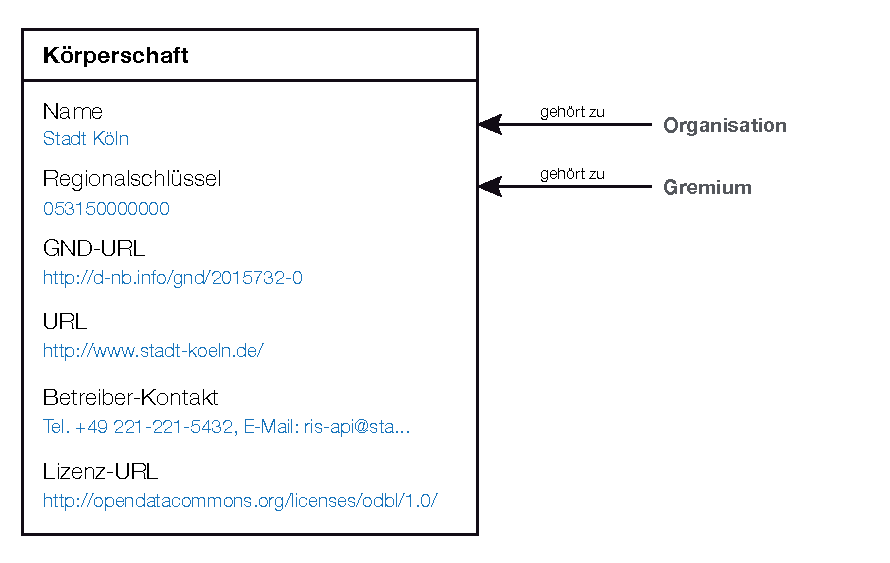
\includegraphics{images/datenmodell_koerperschaft.png}
\caption{Objekttyp Körperschaft}
\end{figure}

\subsubsection{Eindeutige Identifizierung}

Die Körperschaft hat eine innerhalb des Systems eindeutige ID.

Darüber hinaus werden verschiedene Möglichkeiten geboten, die
Körperschaft semantisch zu repräsentieren.

Handelt es sich beim Betreiber des Systems um eine Gebietskörperschaft
(Landkreis, Kommune etc.), soll für die eindeutige Identifizierung der
Regionalschlüssel{[}1{]} verwendet werden.

Darüber hinaus soll zusätzlich, sofern vorhanden, die eindeutige Kennung
der Körperschaft aus der GND{[}12{]} verwendet werden.

Als dritte Möglichkeit, die Körperschaft zu identifizieren, kann eine
aussagekräftigen URL, unter der weitere Informationen zur Körperschaft
zu finden sind, genannt werden.

Sämtliche hier genannten Methoden zur Identifizierung können kombiniert
werden.

\subsubsection{Eigenschaften}

\begin{description}
\item[Schlüssel (\texttt{id})]
Zur eindeutigen Identifizierung der Körperschaft im System
\item[Name (\texttt{name})]
Der Name der Körperschaft, z.B. ``Stadt Köln''
\item[Regionalschlüssel (\texttt{regionalschluessel})]
\emph{Optional}. Regionalschlüssel der Gebietskörperschaft, z.B.
``053150000000''. Muss grundsätzlich 12-stellig angegeben werden.
\item[GND URL (\texttt{gnd\_url})]
\emph{Optional}. URL des Eintrags in der GND, z.B.
``http://d-nb.info/gnd/2015732-0''
\item[URL (\texttt{url})]
\emph{Optional}. URL der Homepage oder einer vergleichbaren Seite mit
Informationen über die Körperschaft, z.B. ``http://www.stadt-koeln.de/''
\item[Lizenz (\texttt{license\_url})]
\emph{Optional}. URL der Lizenz, unter der die Daten, die über die API
abgerufen werden können, stehen.
\item[Betreiber-Kontakt (\texttt{operator\_contact})]
\emph{Optional}. Kontaktinformationen für die direkte Kontaktaufnahme
zum Betreiber der API.
\end{description}

\subsubsection{Beziehungen}

\begin{itemize}
\item
  Objekte vom Typ ``Organisation'' sind zwingend genau einer
  Körperschaft zugeordnet. So wird beispielseise eine SPD in Köln von
  einer SPD in Leverkusen unterschieden.
\item
  Objekte vom Typ ``Gremium'' sind zwingend genau einer Körperschaft
  zugeordnet. Damit wird der ``Rat'' einer bestimmten Kommune von den
  gleichnamigen Gremien anderer Kommunen abgegrenzt.
\end{itemize}

\subsubsection{Beispiel}

\begin{Shaded}
\begin{Highlighting}[]
\NormalTok{\{}
    \DataTypeTok{"id"}\NormalTok{: }\StringTok{"1"}\NormalTok{,}
    \DataTypeTok{"name"}\NormalTok{: }\StringTok{"Stadt Köln"}\NormalTok{,}
    \DataTypeTok{"regionalschluessel"}\NormalTok{: }\StringTok{"053150000000"}\NormalTok{,}
    \DataTypeTok{"gnd_url"}\NormalTok{: }\StringTok{"http://d-nb.info/gnd/2015732-0"}\NormalTok{,}
    \DataTypeTok{"url"}\NormalTok{: }\StringTok{"http://www.stadt-koeln.de/"}\NormalTok{,}
    \DataTypeTok{"operator_contact"}\NormalTok{: }\StringTok{"Tel. +49 221-221-5432, E-Mail: ris-api@stadt-koeln.de"}\NormalTok{,}
    \DataTypeTok{"license_url"}\NormalTok{: }\StringTok{"http://opendatacommons.org/licenses/odbl/1.0/"}
\NormalTok{\}}
\end{Highlighting}
\end{Shaded}

\subsection{Gremium (\emph{committee})}

Das Gremium ist ein Personenkreis, üblicherweise von gewählten und/oder
ernannten Mitgliedern. Beispiele hierfür sind der Stadtrat, Kreisrat,
Gemeinderat, Ausschüsse und Bezirksvertretungen. Gremien halten
Sitzungen ab, zu denen die Gremien-Mitglieder eingeladen werden.

\begin{figure}[htbp]
\centering
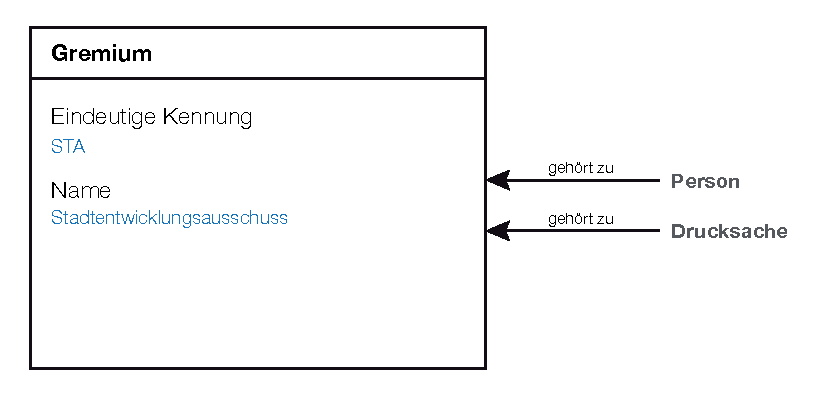
\includegraphics{images/datenmodell_gremium.png}
\caption{Objekttyp Gremium}
\end{figure}

\subsubsection{Eigenschaften}

\begin{description}
\item[Schlüssel (\texttt{id})]
Zur eindeutigen Identifizierung des Gremiums im Kontext einer bestimmten
Körperschaft. In der Praxis kommen sowohl numerische IDs als auch
Namenskürzel (Beispiel: ``STA'' für den Stadtentwicklungsausschuss) vor.
Beides sollte hier Verwendung finden können.
\item[Name (\texttt{name})]
Der Name des Gremiums. Beispiele: ``Rat'', ``Hauptausschuss'',
``Bezirksvertretung 1 (Innenstadt)''
\item[Kurzname (\texttt{short\_name})]
\emph{Optional}. Eine zur Anzeige bestimmte, kürzere Form des Namens.
\item[Zuletzt geändert (\texttt{last\_modified})]
Datum und Uhrzeit der letzten Änderung
\end{description}

\subsubsection{Beziehungen}

\begin{itemize}
\item
  Objekte vom Typ ``Person'' referenzieren auf Gremien, um die
  Mitgliedschaft/Zugehörigkeit einer Person im/zum Gremium zu
  kennzeichnen. Diese Beziehung ist datiert. Das bedeutet, sie hat einen
  Anfangszeitpunkt und ggf. einen Endzeitpunkt.
\item
  Objekte vom Typ ``Drucksache'' verweisen auf Gremien. Beispielsweise
  wird eine Anfrage oder ein Antrag dem Rat und/oder einer bestimmten
  Bezirksvertretung zugeordnet. Details zu dieser Beziehung werden unter
  ``Drucksache'' erläutert.
\item
  Das Gremium verweist auf die Körperschaft, zu der das Gremium gehört.
\end{itemize}

\subsubsection{Beispiel}

\begin{Shaded}
\begin{Highlighting}[]
\NormalTok{\{}
    \DataTypeTok{"id"}\NormalTok{: }\StringTok{"7"}\NormalTok{,}
    \DataTypeTok{"name"}\NormalTok{: }\StringTok{"Finanzausschuss"}\NormalTok{,}
    \DataTypeTok{"short_name"}\NormalTok{: }\StringTok{"FA"}\NormalTok{,}
    \DataTypeTok{"body"}\NormalTok{: }\StringTok{"1"}\NormalTok{,}
    \DataTypeTok{"last_modified"}\NormalTok{: }\StringTok{"2012-08-16T14:05:27+02:00"}
\NormalTok{\}}
\end{Highlighting}
\end{Shaded}

\subsection{Person (\emph{person})}

Jede natürliche Person, die Mitglied eines Gremiums ist, ist als Person
im Datenmodell eindeutig identifizierbar.

\begin{figure}[htbp]
\centering
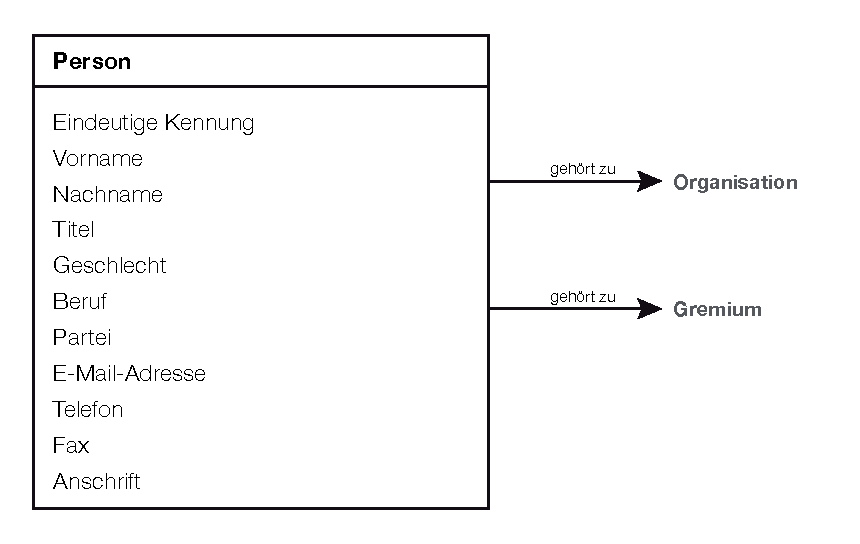
\includegraphics{images/datenmodell_person.png}
\caption{Objekttyp Person}
\end{figure}

\subsubsection{Eigenschaften}

\begin{description}
\item[Schlüssel (\texttt{id})]
Zur eindeutigen Identifizierung sollte jede Person eine Kennung
besitzen, die keinen Änderungen unterworfen ist und aus diesem Grund
nicht mit dem Namen in Verbindung stehen sollte. Viele RIS nutzen rein
numerische Kennungen.
\item[Vorname (\texttt{first\_name})]
Der Vorname der Person.
\item[Nachname (\texttt{last\_name})]
Der Nachname der Person.
\item[Titel (\texttt{academic\_title})]
\emph{Optional}. Akademische Titel wie ``Dr.'' und ``Prof.~Dr.''
\item[Geschlecht (\texttt{sex})]
\emph{Optional}. Weiblich (Wert \texttt{F} für \emph{female}), männlich
(Wert \texttt{M} für \emph{male}), anderes (Wert \texttt{O} für
\emph{others})
\item[Beruf (\texttt{profession})]
\emph{Optional}. Z.B. ``Rechtsanwalt''
\item[E-Mail-Adresse (\texttt{email})]
\emph{Optional}.
\item[Telefon (\texttt{phone})]
\emph{Optional}.
\item[Fax (\texttt{fax})]
\emph{Optional}.
\item[Anschrift (\texttt{address})]
\emph{Optional}. Straße und Hausnummer, Postleitzahl und Ort
\item[Zuletzt geändert (\texttt{last\_modified})]
Datum und Uhrzeit der letzten Änderung
\end{description}

\paragraph{Anmerkungen}

\begin{itemize}
\item
  Das System von Euskirchen scheint Vor- und Nachname (evtl. einschl.
  Titel) in einem gemeinsamen Feld ``Name'' zu führen. Ob das System
  hier technisch differenziert, ist unklar. Falls einzelne Systeme den
  angezeigten Namen nur als ganzes speichern, sollte dies für den
  Standard übernommen werden, da es für die meisten Anwendungen
  ausreichen sollte.
\item
  Das System PROVOX unterscheidet zwischen privaten und geschäftlichen
  Anschriften.
\end{itemize}

\subsubsection{Beziehungen}

\begin{itemize}
\item
  Objekte vom Typ ``Person'' können einer Organisation, z.B. einer
  Fraktion, zugeornet werden. Diese Beziehung ist datiert.
\item
  Objekte vom Typ ``Person'' können einem oder mehreren Gremien
  zugewiesen werden, um die Mitgliedschaft in diesem Gremium
  darzustellen. Diese Beziehungen sind ebenfalls datiert.
\end{itemize}

\subsubsection{Beispiel}

\begin{Shaded}
\begin{Highlighting}[]
\NormalTok{\{}
    \DataTypeTok{"id"}\NormalTok{: }\StringTok{"1000"}\NormalTok{,}
    \DataTypeTok{"first_name"}\NormalTok{: }\StringTok{"Max"}\NormalTok{,}
    \DataTypeTok{"last_name"}\NormalTok{: }\StringTok{"Mustermann"}\NormalTok{,}
    \DataTypeTok{"academic_title"}\NormalTok{: }\StringTok{"Dr."}\NormalTok{,}
    \DataTypeTok{"sex"}\NormalTok{: }\StringTok{"M"}\NormalTok{,}
    \DataTypeTok{"profession"}\NormalTok{: }\StringTok{"Rechtsanwalt"}\NormalTok{,}
    \DataTypeTok{"email"}\NormalTok{: }\StringTok{"max@mustermann.de"}\NormalTok{,}
    \DataTypeTok{"phone"}\NormalTok{: }\StringTok{"+4977777"}\NormalTok{,}
    \DataTypeTok{"fax"}\NormalTok{: }\StringTok{"+4988888"}\NormalTok{,}
    \DataTypeTok{"address"}\NormalTok{: }\StringTok{"Musterstraße 5, 11111 Musterort"}\NormalTok{,}
    \DataTypeTok{"last_modified"}\NormalTok{: }\StringTok{"2012-08-16T14:05:27+02:00"}\NormalTok{,}
    \DataTypeTok{"organisations"}\NormalTok{: [}
        \NormalTok{\{}
            \DataTypeTok{"id"}\NormalTok{: }\StringTok{"2000"}\NormalTok{,}
            \DataTypeTok{"start"}\NormalTok{: }\StringTok{"2011-03-01"}\NormalTok{,}
            \DataTypeTok{"end"}\NormalTok{: }\StringTok{"2013-02-28"}
        \NormalTok{\},}
        \NormalTok{\{}
            \DataTypeTok{"id"}\NormalTok{: }\StringTok{"2001"}\NormalTok{,}
            \DataTypeTok{"start"}\NormalTok{: }\StringTok{"2013-03-01"}
        \NormalTok{\}}
    \NormalTok{],}
    \DataTypeTok{"committees"}\NormalTok{: [}
        \NormalTok{\{}
            \DataTypeTok{"id"}\NormalTok{: }\StringTok{"7"}\NormalTok{,}
            \DataTypeTok{"start"}\NormalTok{: }\StringTok{"2013-01-01"}
        \NormalTok{\}}
    \NormalTok{]}
\NormalTok{\}}
\end{Highlighting}
\end{Shaded}

\subsection{Organisation (\texttt{organisation})}

Organisationen sind üblicherweise Parteien bzw. Fraktionen, denen die
Personen angehören können.

\begin{figure}[htbp]
\centering
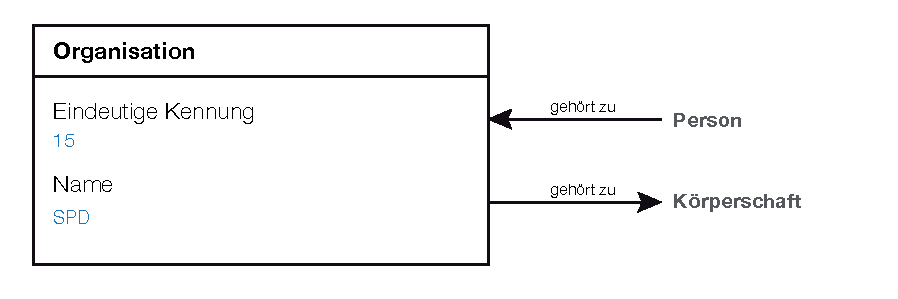
\includegraphics{images/datenmodell_organisation.png}
\caption{Objekttyp Organisation}
\end{figure}

\subsubsection{Eigenschaften}

\begin{description}
\item[Schlüssel (\texttt{id})]
Zur eindeutigen Kennzeichnung einer Organisation innerhalb des Systems
\item[Name (\texttt{name})]
Der gebräuchliche Name der Organisation, z.B. ``SPD'' oder ``DIE
LINKE''.
\item[Zuletzt geändert (\texttt{last\_modified})]
Datum und Uhrzeit der letzten Änderung
\end{description}

\paragraph{Anmerkungen}

\begin{itemize}
\item
  Unklar ist bislang, ob Organisationen in der Praxis eher Fraktionen
  (``SPD-Fraktion im Kölner Rat'', ``SPD-Fraktion in Köln-Innenstadt'')
  abbilden oder ob eher Ortsverbände von Parteien (``SPD Köln'') gemeint
  sein werden. Einblicke, wie gängige Systeme dies handhaben, sollten
  evtl. gesammelt und berücksichtigt werden.
\end{itemize}

\subsubsection{Beziehungen}

\begin{itemize}
\item
  Jede Organisationen gehört zu einer Körperschaft.
\item
  Personen können Organisationen angehören (\emph{datiert}).
\end{itemize}

\subsubsection{Beispiel}

\begin{Shaded}
\begin{Highlighting}[]
\NormalTok{\{}
    \DataTypeTok{"id"}\NormalTok{: }\StringTok{"15"}\NormalTok{,}
    \DataTypeTok{"name"}\NormalTok{: }\StringTok{"SPD"}\NormalTok{,}
    \DataTypeTok{"body"}\NormalTok{: }\StringTok{"1"}\NormalTok{,}
    \DataTypeTok{"last_modified"}\NormalTok{: }\StringTok{"2012-08-16T14:05:27+02:00"}
\NormalTok{\}}
\end{Highlighting}
\end{Shaded}

\subsection{Sitzung (\texttt{meeting})}

Eine Sitzung ist die Versammlung der Mitglieder eines Gremiums oder
mehrerer Gremien zu einem bestimmten Zeitpunkt an einem bestimmten Ort.

Die geladenen Teilnehmer der Sitzung sind jeweils als „Person`` in
entsprechender Form referenziert. Verschiedene Dokumente (Einladung,
Ergebnis- und Wortprotokoll, sonstige Anlagen) können referenziert
werden.

\begin{figure}[htbp]
\centering
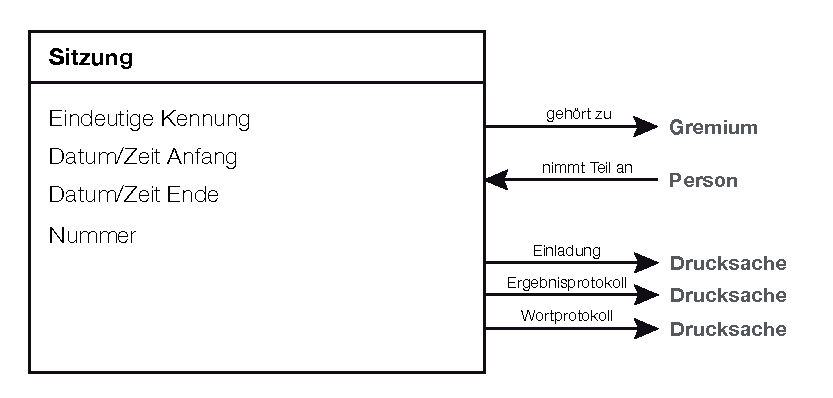
\includegraphics{images/datenmodell_sitzung.png}
\caption{Objekttyp Sitzung}
\end{figure}

\subsubsection{Eigenschaften}

\begin{description}
\item[Schlüssel (\texttt{id})]
Zur eindeutigen Identifizierung der Sitzung innerhalb des Systems. In
der Praxis wird ein solcher Schlüssel entweder durch eine numerische ID
gebildet oder durch Kombination mehrerer Merkmale wie dem Kürzel des
Gremiums, der laufenden Nummer der Sitzung in einem Jahr und der
Jahreszahl (z.B. ``BV1/0034/2012'').
\item[Nummer (\texttt{sequence\_number})]
\emph{Optional}. Laufende Nummer der Sitzung, üblicherweise innerhalb
der Wahlperiode mit 1 beginnend. In der Praxis wird dadurch z.B. die
``2. Sitzung des Rats'' gekennzeichnet. Ist dieses Feld gesetzt, MUSS
ein numerischer Wert enthalten sein.
\item[Anfang (\texttt{start})]
Datum und ggf. Uhrzeit des Anfangszeitpunkts der Sitzung
\item[Ende (\texttt{end})]
\emph{Optional}. Datum und Uhrzeit vom Ende der Sitzung
\item[Ort (\texttt{address})]
\emph{Optional}. Textliche Information zum Ort der Sitzung, z.B.
``Rathaus, Raum 136''.
\item[Zuletzt geändert (\texttt{last\_modified})]
Datum und Uhrzeit der letzten Änderung
\end{description}

\subsubsection{Beziehungen}

\begin{itemize}
\item
  Sitzungen sind mindestens einem Gremium zugeordnet
\item
  Einer Sitzung sind Personen zugeordnet, um die Teilnahme an der
  Sitzung auszudrücken.
\item
  Dokumente können vom Typ ``Sitzung'' \emph{optional} zu mehreren
  Zwecken referenziert werden:

  \begin{itemize}
  \item
    Zum Verweis auf die Einladung zur Sitzung
  \item
    Zum Verweis auf das Ergebnisprotokoll zur Sitzung
  \item
    Zum Verweis auf das Wortprotokoll zur Sitzung
  \end{itemize}
\item
  Weiterhin können Sitzungen beliebige weitere Dokumente, die keine
  eigenständigen Drucksachen sind, referenzieren. Dabei handelt es sich
  dann um nicht weiter spezifizierte Anlagen.
\end{itemize}

\subsubsection{Beispiel}

\begin{Shaded}
\begin{Highlighting}[]
\NormalTok{\{}
    \DataTypeTok{"id"}\NormalTok{: }\StringTok{"3271"}\NormalTok{,}
    \DataTypeTok{"identifier"}\NormalTok{: }\StringTok{"STA/0034/2012"}\NormalTok{,}
    \DataTypeTok{"start"}\NormalTok{: }\StringTok{"2013-01-04T08:00:00+01:00"}\NormalTok{,}
    \DataTypeTok{"end"}\NormalTok{: }\StringTok{"2013-01-04T12:00:00+01:00"}\NormalTok{,}
    \DataTypeTok{"address"}\NormalTok{: }\StringTok{"Rathaus, Raum 136"}\NormalTok{,}
    \DataTypeTok{"sequence_number"}\NormalTok{: }\DecValTok{1}\NormalTok{,}
    \DataTypeTok{"committees"}\NormalTok{: [}\StringTok{"STA"}\NormalTok{],}
    \DataTypeTok{"people"}\NormalTok{: [}\StringTok{"1000"}\NormalTok{, }\StringTok{"1001"}\NormalTok{],}
    \DataTypeTok{"invitation"}\NormalTok{: }\StringTok{"0001/2013"}\NormalTok{,}
    \DataTypeTok{"result_minutes"}\NormalTok{: }\StringTok{"0002/2013"}\NormalTok{,}
    \DataTypeTok{"verbatim_minutes"}\NormalTok{: }\StringTok{"0003/2013"}\NormalTok{,}
    \DataTypeTok{"attachments"}\NormalTok{: [}
        \StringTok{"0004/2013"}\NormalTok{,}
        \StringTok{"0005/2013"}
    \NormalTok{],}
    \DataTypeTok{"last_modified"}\NormalTok{: }\StringTok{"2012-01-08T14:05:27+01:00"}
\NormalTok{\}}
\end{Highlighting}
\end{Shaded}

\subsection{Tagesordnungspunkt (\texttt{agendaitem})}

Der Tagesordnungspunkt wird für eine bestimmte Sitzung angelegt, erhält
eine (innerhalb dieser Sitzung eindeutige) Nummer und einen Titel
(Betreff). Nach der Sitzung wird dem Tagesordnungspunkt außerdem ein
Ergebnis angehängt. Unter Umständen kann dem Tagesordnungspunkt ein
bestimmter Beschlusstext beigefügt sein.

Überlicherweise haben Sitzungen mehrere Tagesordnungspunkte.

\begin{figure}[htbp]
\centering
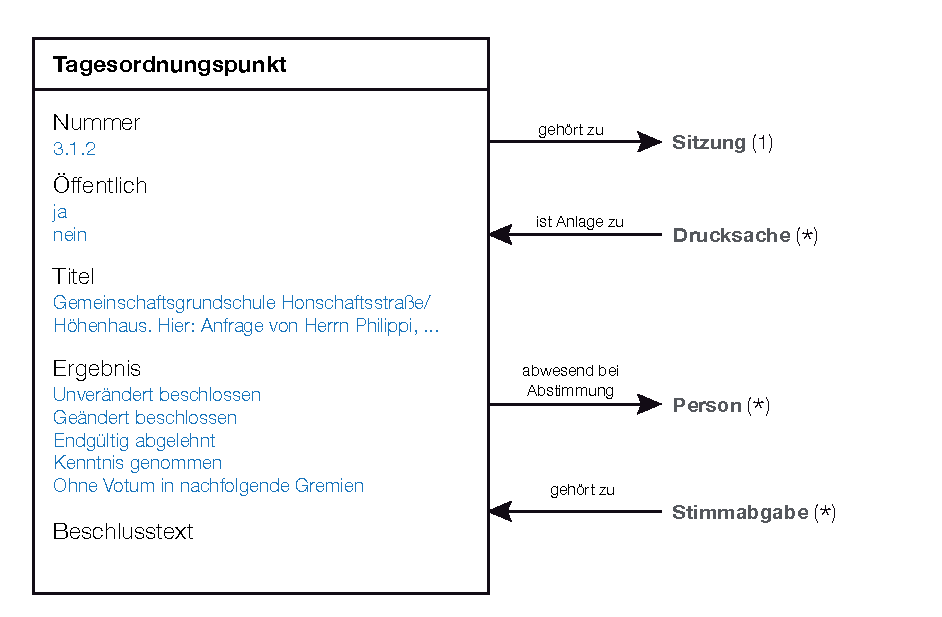
\includegraphics{images/datenmodell_tagesordnungspunkt.png}
\caption{Objekttyp Tagesordnungspunkt}
\end{figure}

\subsubsection{Eigenschaften}

\begin{description}
\item[Nummer (\texttt{identifier})]
Beispiel: ``1.2.3''. Diese Nummer gibt an, in welcher Reihenfolge die
Tagesordnungspunkte einer Sitzung normalerweise behandelt werden. Im
Kontext einer Sitzung ist diese Nummer eindeutig.
\item[Öffentlich (\texttt{public})]
Kennzeichnet, ob der Tagesordnungspunkt in öffentlicher Sitzung
behandelt wird. Kann die Werte \texttt{true} (öffentlich) oder
\texttt{false} annehmen.
\item[Titel (\texttt{title})]
Das Thema des Tagesordnungspunktes
\item[Ergebnis (\texttt{result})]
\emph{Optional}. Kategorische Information darüber, welches Ergebnis die
Beratung des Tagesordnungspunktes gebracht hat. In der Praxis sind hier
Kategorien wie ``Unverändert beschlossen'', ``Geändert beschlossen'',
``Endgültig abgelehnt'', ``Zur Kenntnis genommen'', ``Ohne Votum in
nachfolgende Gremien überwiesen'' und weitere zu erwarten.
\item[Ergebnis Details (\texttt{result\_details})]
\emph{Optional}. Ermöglicht die Angabe zusätzlicher Textinformationen
zum Ergebnis, zum Beispiel im Fall der Verweisung an ein anderes Gremium
die Angabe, an welches Gremium verwiesen wurde.
\item[Beschlusstext (\texttt{resolution\_text})]
\emph{Optional}. Falls in diesem Tagesordnungspunkt ein Beschluss
gefasst wurde, kann der Text hier hinterlegt werden. Das ist besonders
dann in der Praxis relevant, wenn der gefasste Beschluss (z.B. durch
Änderungsantrag) von der Beschlussvorlage abweicht.
\item[Zuletzt geändert (\texttt{last\_modified})]
Datum und Uhrzeit der letzten Änderung
\end{description}

\paragraph{Anmerkungen}

\begin{itemize}
\item
  Einige Systeme vergeben zu Tagesordnungspunkten intern
  unveränderliche, numerische IDs. Es ist unklar, ob es zusätzlichen
  Nutzen bringt, derartige IDs, neben den Nummern, in den Standard zu
  übernehmen. Dies würde vermutlich nur Sinn ergeben, wenn es als
  Pflichtfeld gelten könnte.
\item
  Teil der Beratungen über einheitliche Nomenklatur im Standard sollte
  sein, eine Vereinheitlichung der Werte für die Eigenschaft
  \texttt{result} zu diskutieren.
\end{itemize}

\subsubsection{Beziehungen}

\begin{itemize}
\item
  Jeder Tagesordnungspunkt gehört zu genau einer Sitzung.
\item
  Der Tagesordnungspunkt kann auf eine Drucksache verweisen, die im
  Rahmen dieses Tagesordnungspunkt beraten werden soll.
\item
  Es können Personen referenziert werden, die während der Abstimmung zu
  diesem Tagesordnungspunkt \emph{nicht} anwesend waren.
\end{itemize}

\subsubsection{Beispiel}

\begin{Shaded}
\begin{Highlighting}[]
\NormalTok{\{}
    \DataTypeTok{"meeting"}\NormalTok{: }\StringTok{"3271"}\NormalTok{,}
    \DataTypeTok{"identifier"}\NormalTok{: }\StringTok{"3.1.2"}\NormalTok{,}
    \DataTypeTok{"public"}\NormalTok{: }\DecValTok{true}\NormalTok{,}
    \DataTypeTok{"title"}\NormalTok{: }\StringTok{"Gemeinschaftsgrundschule Hornschaftsstraße/Höhenhaus. Hier: Anfrage von Herrn Philippi"}\NormalTok{,}
    \DataTypeTok{"result"}\NormalTok{: }\StringTok{"Geändert beschlossen"}\NormalTok{,}
    \DataTypeTok{"resolution_text"}\NormalTok{: }\StringTok{"Der Beschluss weicht wie folgt vom Antrag ab: ..."}\NormalTok{,}
    \DataTypeTok{"people_absent"}\NormalTok{: [}\StringTok{"1002"}\NormalTok{, }\StringTok{"1003"}\NormalTok{],}
    \DataTypeTok{"last_modified"}\NormalTok{: }\StringTok{"2012-08-16T14:05:27+02:00"}
\NormalTok{\}}
\end{Highlighting}
\end{Shaded}

\subsection{Drucksache (\texttt{paper})}

Eine Drucksache bildet Mitteilungen, Antworten auf Anfragen,
Beschlussvorlagen, Anfragen, Anträge und weitere Vorlagen ab. Jede
Drucksache erhält eine eindeutige Kennung.

Die Drucksache hat im Informationsmodell eine hervorgehobene Bedeutung.
Im Fall eines Antrags kann mit einer einzigen Drucksache ein über Monate
oder Jahre dauernder politischer Entscheidungsprozess verbunden sein. In
dem Zusammenhang entstehen üblicherweise weitere Drucksachen.

Drucksachen spielen in der schriftlichen wie mündlichen Kommunikation
eine besondere Rolle, da in vielen Texten auf bestimmte Drucksachen
Bezug genommen wird. Hierbei kommen in Ratsinformationssystemen
unveränderliche Kennungen der Drucksachen zum Einsatz.

\begin{figure}[htbp]
\centering
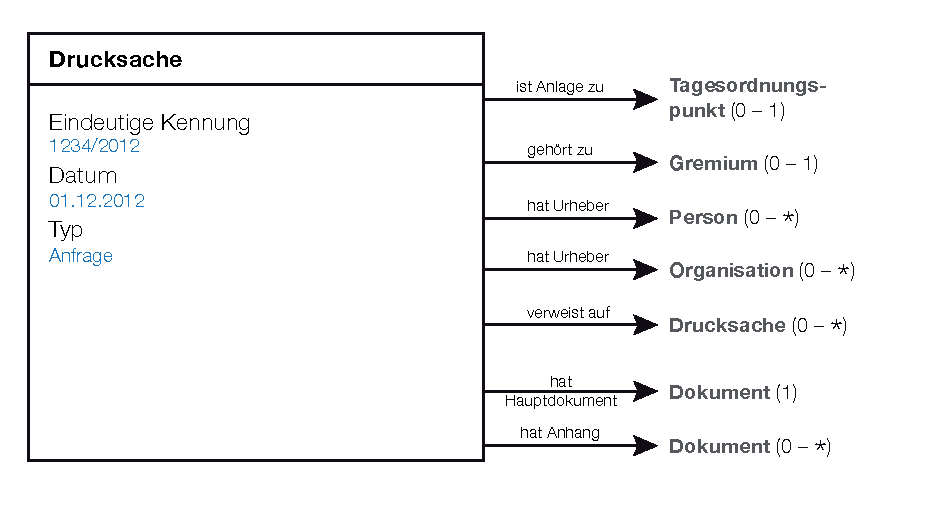
\includegraphics{images/datenmodell_drucksache.png}
\caption{Objekttyp Drucksache}
\end{figure}

Jede Drucksache ist über die Eigenschaft ``Typ'' als eine der folgenden
Arten von Drucksachen gekennzeichnet:

\begin{itemize}
\item
  \textbf{Beschlussvorlage}: Entscheidungsvorschlag der Verwaltung
\item
  \textbf{Antrag}: Entscheidungsvorschlag einer Fraktionen bzw. mehrerer
  Fraktionen oder einer/mehrerer Einzelperson/en
\item
  \textbf{Anfrage}: Frage(n) einer oder mehrerer Fraktion oder
  Einzelpersonen an die Verwaltung
\item
  \textbf{Mitteilung/Stellungnahme der Verwaltung}: Eine Information der
  Verwaltung an einzelne oder mehrere Gremien. Darunter fallen nicht
  Beantwortungen von Anfragen.
\item
  \textbf{Beantwortung einer Anfrage}: Antwort der Verwaltung auf
  (mündliche oder schriftliche) Anfragen
\end{itemize}

\subsubsection{Eigenschaften}

\begin{description}
\item[Schlüssel (\texttt{id})]
Die Kennung einer Drucksache muss für die jeweilige Körperschaft
eindeutig sein. Sie kann sowohl Ziffern als auch Buchstaben enthalten.
Einige Systeme (z.B. Köln) verwenden besondere Trennzeichen wie ``/'',
um eine Jahreszahl von einer laufenden Nummer abzutrennen. Weiterhin
werden mancherorts führende Nullen verwendet.
\item[Datum (\texttt{date})]
Datum der Veröffentlichung
\item[Typ (\texttt{type})]
Art der Drucksache (Erläuterung siehe oben)
\item[Zuletzt geändert (\texttt{last\_modified})]
Datum und Uhrzeit der letzten Änderung
\end{description}

\subsubsection{Beziehungen}

\begin{itemize}
\item
  Es muss genau ein \textbf{Hauptdokument} (Objekttyp ``Dokument'')
  referenziert werden.
\item
  Es können beliebig viele weitere Dokumente referenziert werden, die
  als nachgeordnete \textbf{Anlagen} zur Drucksache verstanden werden.
\item
  Die Drucksache ist beliebig vielen Gremien zuzuordnen, in denen diese
  beraten wird.
\item
  Drucksachen können \textbf{Urhebern} zugewiesen werden. Im Fall von
  Mitteilungen der Verwaltung ist dies oft der Oberbürgermeister. Bei
  Anträgen oder Anfragen können Organisationen oder Einzelpersonen
  referenziert werden. Es können stets mehrere Uhrheber verknüpft
  werden.
\item
  Es können beliebig viele \textbf{Orte} (siehe Objekttyp ``Ort'')
  referenziert werden, die im Inhalt der Drucksache behandelt werden.
  Beispiel: Beschlussvorlage zur Freigabe von Mitteln für die Sanierung
  eines Sportplatzes, wobei der Ort die Lage des Sportplatzes genau
  beschreibt.
\item
  Drucksachen können auf andere Drucksachen referenzieren. Diese
  Verweise können verschiedene semantische Beziehungen ausdrücken. So
  kann eine Drucksache auf eine übergeordnete oder eine oder mehrere
  untergeordnete Drucksachen verweisen. Beim Drucksachen-Typ
  ``Beantwortung einer Anfrage'' ist die Drucksache zu referenzieren,
  die die ursprüngliche \textbf{Anfrage} beinhaltet. Denkbar sind auch
  Verweise auf frühere Drucksachen zum selben Thema. Zu klären ist, wie
  die verschiedenen möglichen Beziehungen formell ausgedrückt werden.
\item
  Drucksachen können zu beliebig vielen Tagesordnungspunkten in
  Beziehung stehen, um die \textbf{Beratungsfolge} einer Drucksache
  abzubilden. Hierbei kann die Beziehung jeweils mit einer Zuständigkeit
  versehen sein, die noch näher zu bestimmen ist (TODO).
\end{itemize}

\subsubsection{Beispiel}

\begin{Shaded}
\begin{Highlighting}[]
\NormalTok{\{}
    \DataTypeTok{"id"}\NormalTok{: }\StringTok{"1234/2012"}\NormalTok{,}
    \DataTypeTok{"date"}\NormalTok{: }\StringTok{"2013-01-04"}\NormalTok{,}
    \DataTypeTok{"type"}\NormalTok{: }\StringTok{"Beantwortung einer Anfrage"}\NormalTok{,}
    \DataTypeTok{"related_papers"}\NormalTok{: [}
        \StringTok{"0768/2012"}
    \NormalTok{],}
    \DataTypeTok{"main_document"}\NormalTok{: }\StringTok{"3000.pdf"}\NormalTok{,}
    \DataTypeTok{"attachments"}\NormalTok{: [}
        \StringTok{"3002.pdf"}\NormalTok{,}
        \StringTok{"3003.pdf"}
    \NormalTok{],}
    \DataTypeTok{"locations"}\NormalTok{: [}
        \NormalTok{\{}
            \DataTypeTok{"description"}\NormalTok{: }\StringTok{"Theodor-Heuss-Ring 1"}\NormalTok{,}
            \DataTypeTok{"lat"}\NormalTok{: }\FloatTok{7.148}\NormalTok{,}
            \DataTypeTok{"lon"}\NormalTok{: }\FloatTok{50.023}
        \NormalTok{\}}
    \NormalTok{],}
    \DataTypeTok{"committees"}\NormalTok{: [}\StringTok{"STA"}\NormalTok{],}
    \DataTypeTok{"creators"}\NormalTok{: [}
        \NormalTok{\{}
            \DataTypeTok{"typ"}\NormalTok{: }\StringTok{"Organisation"}\NormalTok{,}
            \DataTypeTok{"id"}\NormalTok{: }\StringTok{"2000"}
        \NormalTok{\},}
        \NormalTok{\{}
            \DataTypeTok{"typ"}\NormalTok{: }\StringTok{"Person"}\NormalTok{,}
            \DataTypeTok{"id"}\NormalTok{: }\StringTok{"1000"}
        \NormalTok{\}}
    \NormalTok{],}
    \DataTypeTok{"consultations"}\NormalTok{: [}
        \NormalTok{\{}
            \DataTypeTok{"meeting"}\NormalTok{: }\StringTok{"3271"}\NormalTok{,}
            \DataTypeTok{"agendaitem"}\NormalTok{: }\StringTok{"3.1.2"}\NormalTok{,}
            \DataTypeTok{"role"}\NormalTok{: }\StringTok{"Federführende Beratung"}
        \NormalTok{\}}
    \NormalTok{],}
    \DataTypeTok{"last_modified"}\NormalTok{: }\StringTok{"2013-01-08T12:05:27+01:00"}
\NormalTok{\}}
\end{Highlighting}
\end{Shaded}

\subsection{Dokument (\texttt{document})}

Ein Dokument hält die Metadaten einer Datei vor, beispielsweise einer
PDF-Datei, eines RTF- oder Word-Dokuments.

Wird von einem Word-Dokument eine PDF-Ableitung hinterlegt, ist diese
Ableitung ebenfalls ein Dokument. Um zu zeigen, dass es sich um eine
Ableitung handelt, verweist dieses auf das Original als ``Master''.

Im Unterschied zur Drucksache benötigt das Dokument keine
nutzerfreundliche Kennung.

\begin{figure}[htbp]
\centering
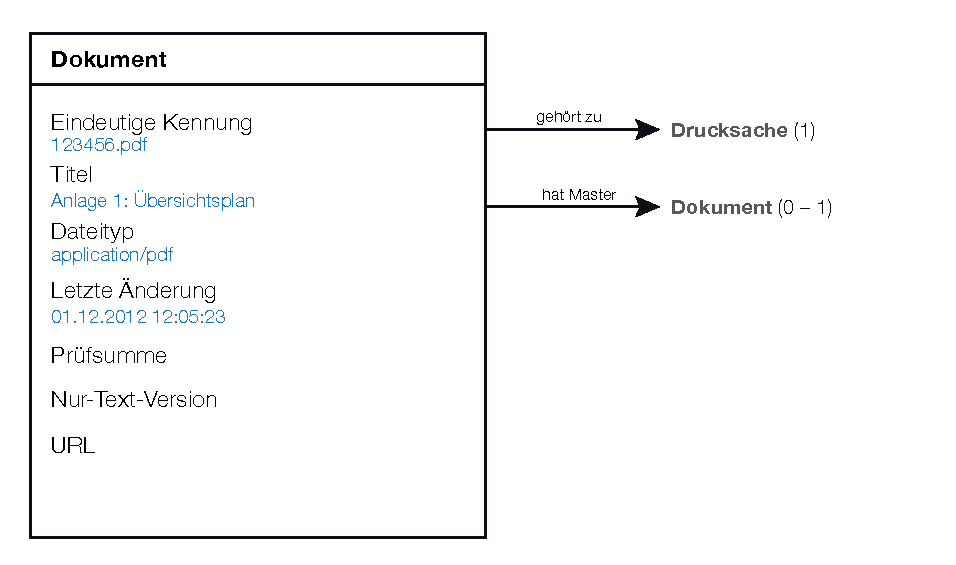
\includegraphics{images/datenmodell_dokument.png}
\caption{Objekttyp Dokument}
\end{figure}

\subsubsection{Eigenschaften}

\begin{description}
\item[Schlüssel (\texttt{id})]
Unveränderliche Kennung
\item[Name (\texttt{name})]
Dateiname, z.B. ``12345.pdf''
\item[Dateityp (\texttt{mime\_type})]
Mime-Typ des Inhalts, z.B. ``application/pdf''
\item[Veröffentlichungsdatum (\texttt{date})]
Datum des Tages, an dem das Dokument ins System eingestellt wurde
\item[Änderungsdatum und -uhrzeit (\texttt{last\_modified})]
Datum und Uhrzeit der letzten Änderung des Dokuments
\item[Prüfsumme (\texttt{sha1\_checksum})]
SHA1-Prüfsumme des Dokumenteninhalts
\item[URL (\texttt{url})]
URL zum Abruf der Daten dieses Dokuments mittels HTTP GET-Aufruf
\item[Nur-Text-Version (\texttt{text})]
Reine Text-Wiedergabe des Dokumenteninhalts, sofern es sich nicht um
eine reine Abbildung handelt.
\end{description}

\subsubsection{Beziehungen}

\begin{itemize}
\item
  Dokumente gehören zwingend zu einer \textbf{Drucksache}, optional auch
  zu mehreren. Ein Dokument kann entweder als Hauptdokument einer
  Drucksache oder als Anlage eingestuft sein.
\item
  Ein Dokument kann auf ein anderes Dokument referenzieren, wenn es von
  dem anderen Dokument abstammt. So ist es möglich, von einem
  abgeleiteten Dokument zu seinem Dokumenten-Master zu gelangen
  (Beispiel: von einem PDF-Dokument zum OpenOffice-Original).
\end{itemize}

\begin{Shaded}
\begin{Highlighting}[]
\NormalTok{\{}
    \DataTypeTok{"id"}\NormalTok{: }\StringTok{"3000"}\NormalTok{,}
    \DataTypeTok{"name"}\NormalTok{: }\StringTok{"3000.pdf"}\NormalTok{,}
    \DataTypeTok{"mime_type"}\NormalTok{: }\StringTok{"application/pdf"}\NormalTok{,}
    \DataTypeTok{"date"}\NormalTok{: }\StringTok{"2013-01-04T07:54:13+01:00"}\NormalTok{,}
    \DataTypeTok{"last_modified"}\NormalTok{: }\StringTok{"2013-01-04T07:54:13+01:00"}\NormalTok{,}
    \DataTypeTok{"sha1_checksum"}\NormalTok{: }\StringTok{"da39a3ee5e6b4b0d3255bfef95601890afd80709"}\NormalTok{,}
    \DataTypeTok{"url"}\NormalTok{: }\StringTok{"http://ris.beispielstadt.de/api/documents/3000.pdf"}\NormalTok{,}
    \DataTypeTok{"text"}\NormalTok{: }\StringTok{"Der Übersichtsplan zeigt alle Ebenen des ..."}\NormalTok{,}
    \DataTypeTok{"master"}\NormalTok{: }\StringTok{"2099"}
\NormalTok{\}}
\end{Highlighting}
\end{Shaded}

\subsection{Ort (\texttt{location})}

Dieser Objekttyp dient dazu, einen Ortsbezug einer Drucksache formal
abzubilden. Ortsangaben können sowohl aus Textinformationen bestehen
(beispielsweise der Name einer Straße/eines Platzes oder eine genaue
Adresse) als auch aus Geodaten.

OParl sieht die Angabe von Geodaten in Anlehnung an die
GeoJSON-Spezifikation {[}13{]} vor. Die GeoJSON-Spezifikation erlaubt
die Abbildung von vielen unterschiedlichen Geometrien wie Punkten,
Pfaden und Polygonen. Während GeoJSON zu jedem Geodaten-Objekt auch die
Speicherung zusätzlicher Metadaten ermöglicht, beschränkt sich OParl
ledliglich auf das \texttt{geometry}-Attribut in GeoJSON. Sämtliche
Geo-Koordinatenangaben werden in in OParl im WGS-84-System {[}11{]}
erwartet.

\begin{figure}[htbp]
\centering
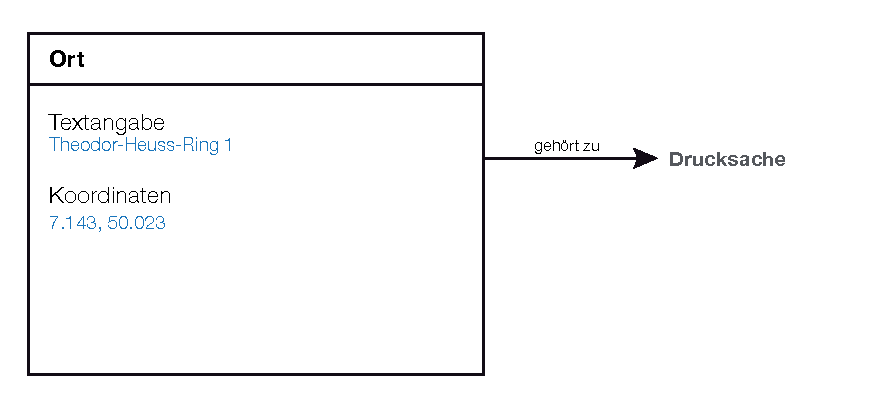
\includegraphics{images/datenmodell_ort.png}
\caption{Objekttyp Ort}
\end{figure}

\subsubsection{Eigenschaften}

\begin{description}
\item[Textanabe (\texttt{description})]
\emph{Optional.} Textliche Beschreibung eines Orts, z.B. in Form einer
Adresse
\item[Koordinaten (\texttt{geometry})]
\emph{Optional.} GeoJSON geometry Objekt
\item[Zuletzt geändert (\texttt{last\_modified})]
Datum und Uhrzeit der letzten Änderung
\end{description}

\subsubsection{Beziehungen}

\begin{itemize}
\item
  Orte können mit Drucksachen in Verbindung stehen.
\end{itemize}

\begin{Shaded}
\begin{Highlighting}[]
\NormalTok{\{}
    \DataTypeTok{"description"}\NormalTok{: }\StringTok{"Honschaftsstraße 312, 51061 Köln"}\NormalTok{,}
    \DataTypeTok{"geometry"}\NormalTok{: \{}
        \DataTypeTok{"type"}\NormalTok{: }\StringTok{"Point"}\NormalTok{,}
        \DataTypeTok{"coordinates"}\NormalTok{: [}\FloatTok{7.03291}\NormalTok{, }\FloatTok{50.98249}\NormalTok{]}
    \NormalTok{\},}
    \DataTypeTok{"last_modified"}\NormalTok{: }\StringTok{"2013-02-14T14:05:27+01:00"}
\NormalTok{\}}
\end{Highlighting}
\end{Shaded}

\section{Fußnoten}

{[}1{]}: Siehe
\href{http://de.wikipedia.org/wiki/Amtlicher\_Gemeindeschl\%C3\%BCssel}{de.wikipedia.org/wiki/Amtlicher\_Gemeindeschlüssel}

{[}2{]}: Ratsinformationssystem der Stadt Köln,
\href{http://ratsinformation.stadt-koeln.de/}{http://ratsinformation.stadt-koeln.de/}

{[}3{]}: Firma Somacos,
\href{http://www.somacos.de/de/sitzungsdienst/ratsinfo.html}{SessionNet
Produktinformation}

{[}4{]}: Ratsinformationssystem der Bezirksverwaltugn Berlin Mitte,
\href{http://www.berlin.de/ba-mitte/bvv-online/allris.net.asp}{http://www.berlin.de/\ldots{}}

{[}5{]}: CC e-gov GmbH, \href{http://www.cc-egov.de/allris.htm}{ALLRIS
Produktionformationen}

{[}6{]}: Ratsinformationssystem der Stadt Rösrath,
\href{http://212.227.97.55/ratsinfo/roesrath}{http://212.227.97.55/\ldots{}}

{[}7{]}: \href{http://www.provox.de/}{Firma PROVOX}

{[}8{]}: Ratsinformationssystem der Stadt Euskirchen,
\href{https://sitzungsdienst.euskirchen.de/}{https://sitzungsdienst.euskirchen.de/}

{[}9{]}: Firma Sternberg,
\href{http://www.sitzungsdienst.net/produkte/ratsinformationsmanagement}{SD.NET
RIM Produktionformationen}

{[}10{]}: BoRis, Ratsinformationssystem der Stadt Bonn
(Eigenentwicklung).
\href{http://www2.bonn.de/bo\_ris/ris\_sql/agm\_index.asp}{http://www2.bonn.de/\ldots{}}

{[}11{]}: World Geodetic System 1984 (EPSG:4326), wird unter anderem
auch vom Global Positioning System (GPS) verwendet.

{[}12{]}: Gemeinsame Normdatei:
\href{http://de.wikipedia.org/wiki/Gemeinsame\_Normdatei}{de.wikipedia.org/wiki/Gemeinsame\_Normdatei}

{[}13{]}: GeoJSON \href{http://www.geojson.org/}{www.geojson.org}

{[}14{]}: Frankfurt Gestalten
\href{http://www.geojson.org/}{www.geojson.org}

{[}15{]}: Offenes Köln \href{http://offeneskoeln.de/}{offeneskoeln.de}

{[}16{]}: OpenRuhr:RIS
\href{http://openruhr.de/openruhrris/}{openruhr.de/openruhrris}

\section{Glossar}

\begin{description}
\item[JSON-LD]
JSON for Linked Data
\item[RIS]
Ratsinformationssystem
\item[WGS 84]
World Geodetic System 1984. Ein weltweites Referenzsystem für die
Interpretation von Geokoordinaten-Angaben.
\end{description}

\end{document}
